\section{Motivation}

In the field of psychology and biology, it is widely accepted that in a video display, user-perceived quality is very different from original video quality. It is mainly caused by human visual system [] and human brain signal processing system [].

In this section we show that current rate allocation strategies in VR streaming is far from optimizing user-perceived quality. If we can rightly allocate bitrate for each part of video to maximize user-perceived quality, we can save 50\% bandwidth in the same user-perceived quality, compared with state-of-art methods.

\subsection{Current VR streaming solutions}

In this section we briefly introduce two widely-used VR streaming solutions: monolithic streaming and viewport-driven streaming.

\subsubsection{Monolithic streaming}

Monolithic streaming is a widely used scheme in many VR video providers (e.g. IQiyi, Youku, ...). In monolithic streaming, it is assumed that user-perceived quality is rightly equal to video quality. A VR video is considered the same as a traditional non-VR video, so each spatial part of video is allocated to one same bitrate level. Client chooses a proper bitrate for the whole video chunk according to bandwidth throughput, buffer or other factors.

Monolithic streaming's biggest advantage is easy deployment. Since it deliveries VR video as non-VR video, there is no need to change the video streaming protocol. It can be directly applied on current video streaming system.

The disadvantage of monolithic streaming is obvious. Since in a VR video display, most area of video is out of user's viewport, which are absolutely not viewed by user. Monolithic streaming allocate the same quality level for both in-viewport part and out-viewport part. So it causes serious waste of bandwidth. 

\subsubsection{Viewpoint-driven streaming}
Many user studies have proved that perceived quality of an object in a video is highly related to its distance to user viewpoint. When an object is near to user viewpoint, it should be allocated high bitrate since user is sensitive to its distortion. When an object is far from user viewpoint, it should be allocated low bitrate since distortion is difficult to be noticed.

Viewpoint-driven streaming allocates bitrate for each object in a video based on its distance to user viewpoint. Video is usually cut into several spatial tiles, which can be independently encoded / decoded. Then it can decide the bitrate in tile-level granularity.

In addition, viewpoint prediction technology is needed in viewpoint-driven streaming, since we need to predict user's viewpoint in the next few seconds. Fortunately, in recent years, viewpoint prediction have been well studied and many solutions can obtain high prediction accuracy.

Compared with monolithic streaming, viewpoint-driven streaming can allocate more bitrate for area near the user's viewpoint so it can save a lot of bandwidth while maintaining the same user-perceived quality.

\subsection{What influences user-perceived quality}
In viewpoint-driven streaming, there is a strong assumption that user-perceived quality is only related to viewpoint-object distance. Although viewpoint-driven streaming saves much bandwidth compared with monolithic streaming, it is still far away from user-perceived quality optimization.

In fact, in a video display, user-perceived quality is also related to many other factors:

\begin{itemize}

\item \emph{Perceived quality is highly related to content luminance.} For a very dark content or a very bright content, user is more difficult to notice the content distortion, thus perceived quality is higher. On the other hand, when a content is of medium lightness, user is more sensitive to its distortion. So the same level distortion causes lower perceived quality.

\item \emph{Perceived quality is also related to texture complexity.} The same degree distortion is more likely to be noticed in a simple texture than in a complex texture. So perceived quality is higher in complex texture. This phenomenon is called texture masking.

\end{itemize}

Moreover, in VR video display, perceived quality is related to some new factors, which are not considered in traditional video display:

\begin{itemize}

\item \emph{Viewpoint moving speed can influence perceived quality.} One of the most highlighted feature of VR video is that users can freely move their viewpoints. According to our data analysis, more than x\% time, user's viewpoint is moving faster than y deg/s. When user moves his / her viewpoint, perceived quality is significantly improved, since user is unable to detect the distortion. []

\item \emph{Depth of Field (DoF) can influence perceived quality.} In VR display, different objects have different DoF and it is simulated by binocular parallax. Objects with small DoF (which are near to user) have greater parallax, and greater parallax leads to difficulty of binocular fusion, thus human's ability of detecting distortion is weaker.

\item \emph{User's light / dark adaptation can influence perceived quality.} When user wears a HMD in VR display, environmental brightness perceived by eyes is totally depended on luminance of video content itself. So when the scene changes dramatically from dark to light or from light to dark, user's ability of detecting distortion will be weaker for a period of time.

\end{itemize}

\subsection{Challenges}
In order to achieve perceived quality driven VR streaming, the core challenge is: perceived quality is related to both video content and user behavior, how to take together both-sides information to maximize the perceived quality. 

For specifically, there are three aspects:

\textbf{Challenge 1: Traditional Human Visual System (HVS) models can not measure perceived quality in VR video display.} 

Perceived quality can be well-measured in traditional video display by building mathematical model from luminance, texture complexity and viewpoint-object distance to perceived quality. However, as we have mentioned, besides these existing factors, perceived quality in VR display is related to several new factors which are never modeled before. Their mathematical relationship to perceived quality, and how these new factors combined with existing factors together influence perceived quality are unknown problems.

\textbf{Challenge 2: Traditional grid-like video tiling scheme performs poorly in perceived quality optimization.} 

To optimize perceived quality, we need to independently allocate bitrate of each spatial part of the video. Grid-like tiling scheme is a widely used method to solve the problem. Video is cut into several rectangular tiles with equal size which can be independently encoded / decoded. So we can allocate different bitrate to different tiles.

However, traditional grid-like tiling performs poorly in perceived quality optimization in two aspects: 

(1) Coarse-grained tiling causes coarse-grained rate allocation, and perceived quality obtained by coarse-grained rate allocation is far from that obtained by fine-grained rate allocation. We encode the video with different rate allocation granularity. We apply PSPNR to measure perceived quality and Fig. \ref{optimalencoding} shows the PSPNR-bandwidth tradeoff. Rate allocation with 3*6 / 6*12 granularity obtains -x\% / -x\% PSPNR compared with 12*24 granularity, this is a significant performance gap in perceived quality optimization.

\begin{figure}
  \centering
  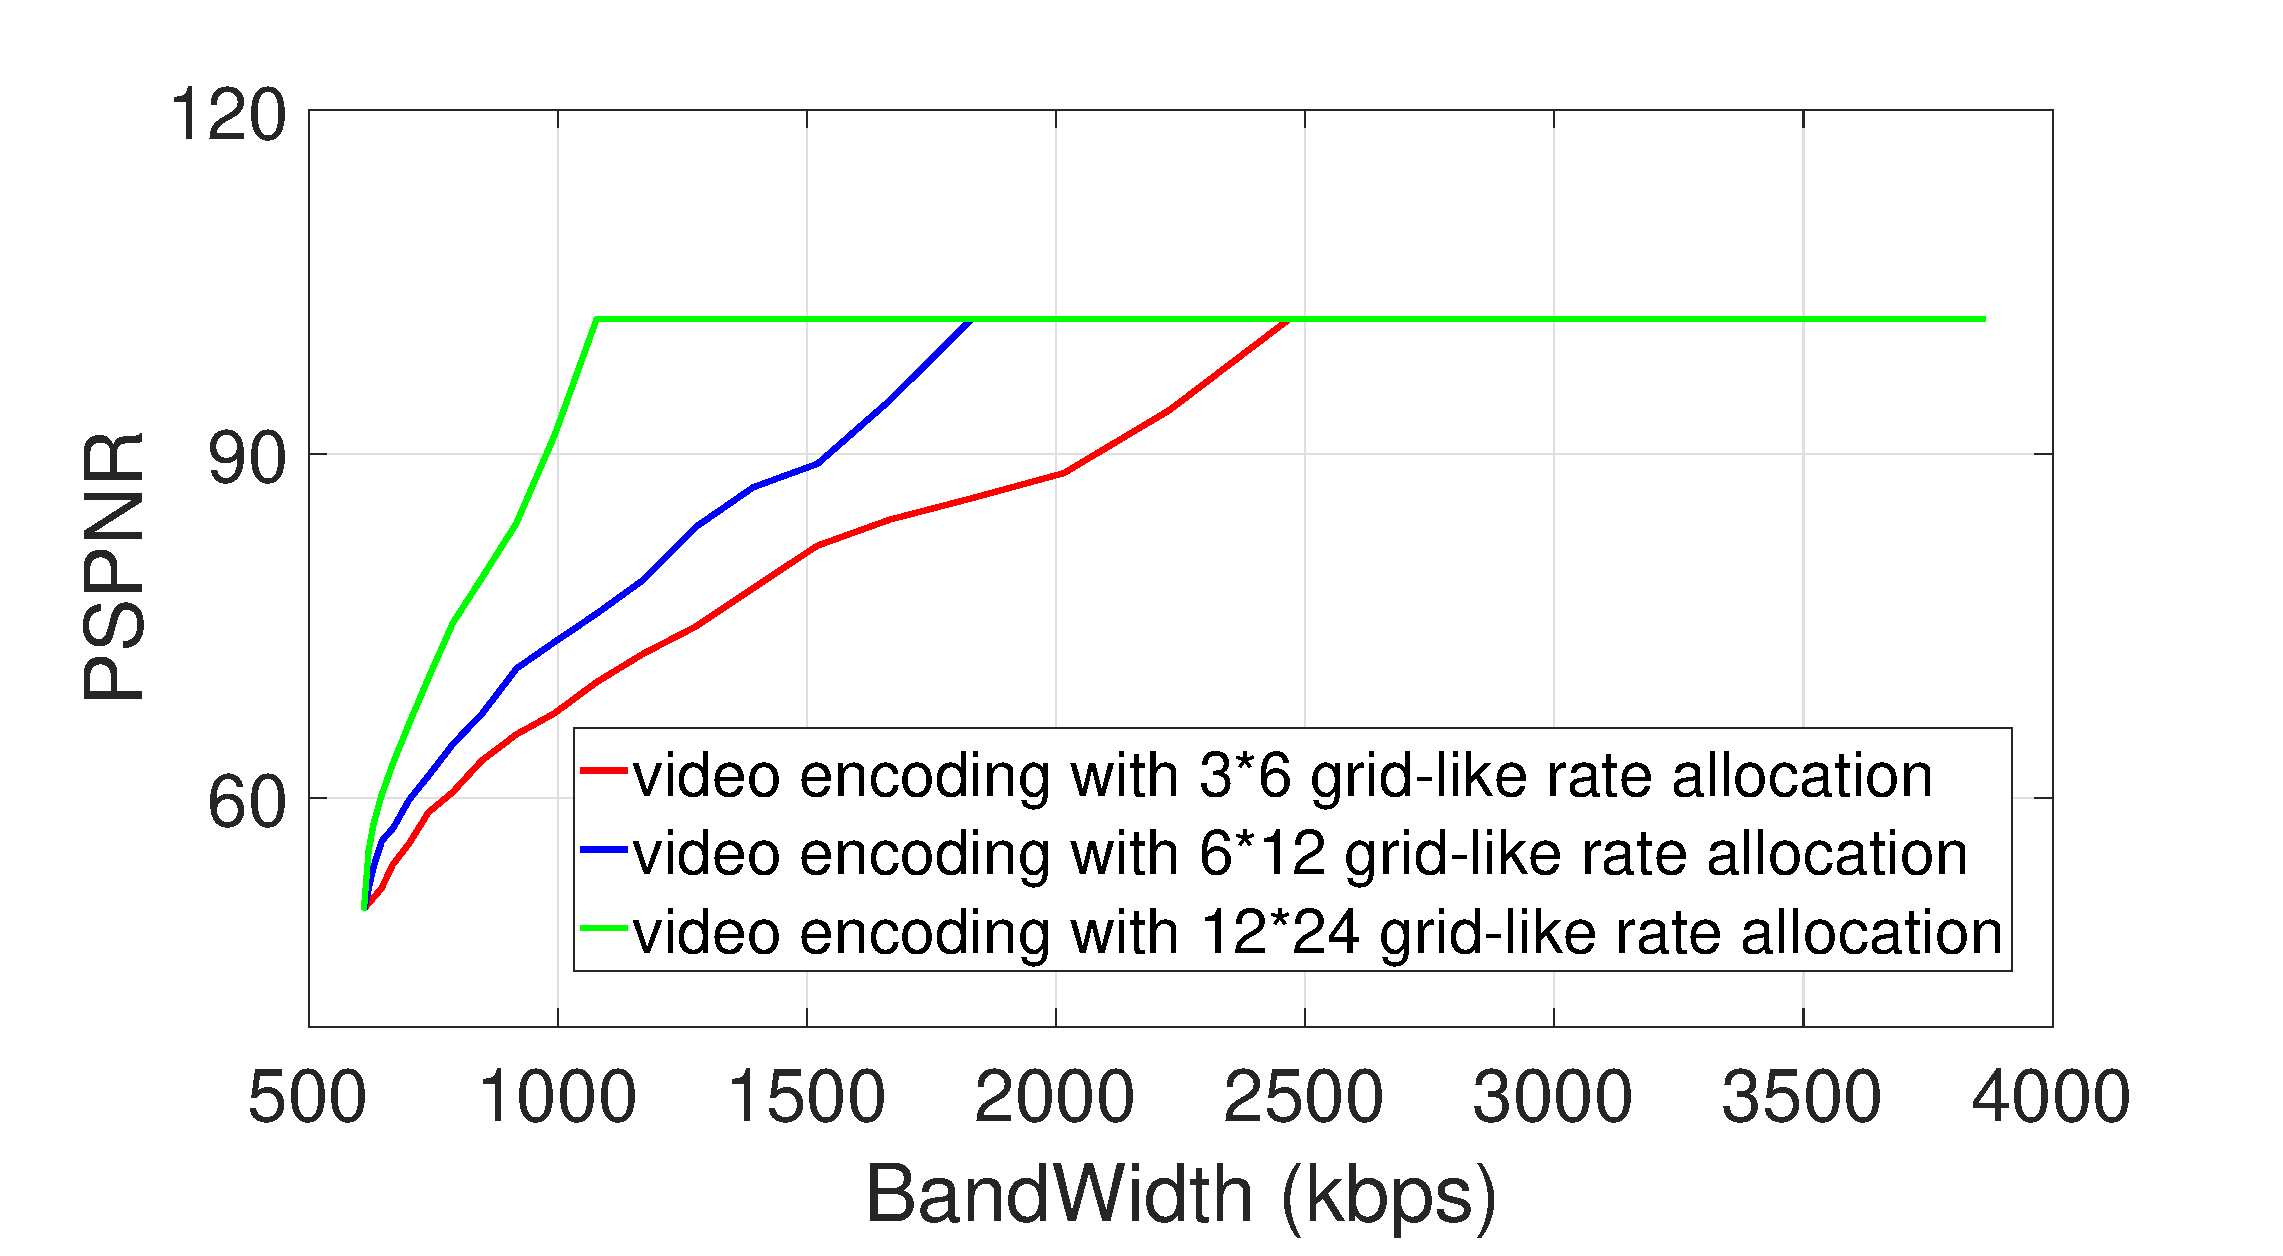
\includegraphics[width=2.5in]{images/optimalencoding.eps}
  \caption{PSPNR-bandwidth tradeoff in video encoding with different granularity of rate allocation.}
  \label{optimalencoding}
  \end{figure}

(2) Fine-grained tiling introduces serious bitrate efficiency problem in video encoding. In practice, each tile has to be encoded independently instead of encoded together. When we cut the video into tiles, the total video size is increased. Fig. \ref{bitrateefficiency} shows the video size of different tiling granularity compared with original video size. We find that cutting a video into 12*24 tiles introduces 50\% to 330\% additional video size compared to original video. This significantly lower its practical performance in perceived quality optimization, especially in low bandwidth situations where the bitrate efficiency problem is very serious.

\begin{figure}
  \centering
  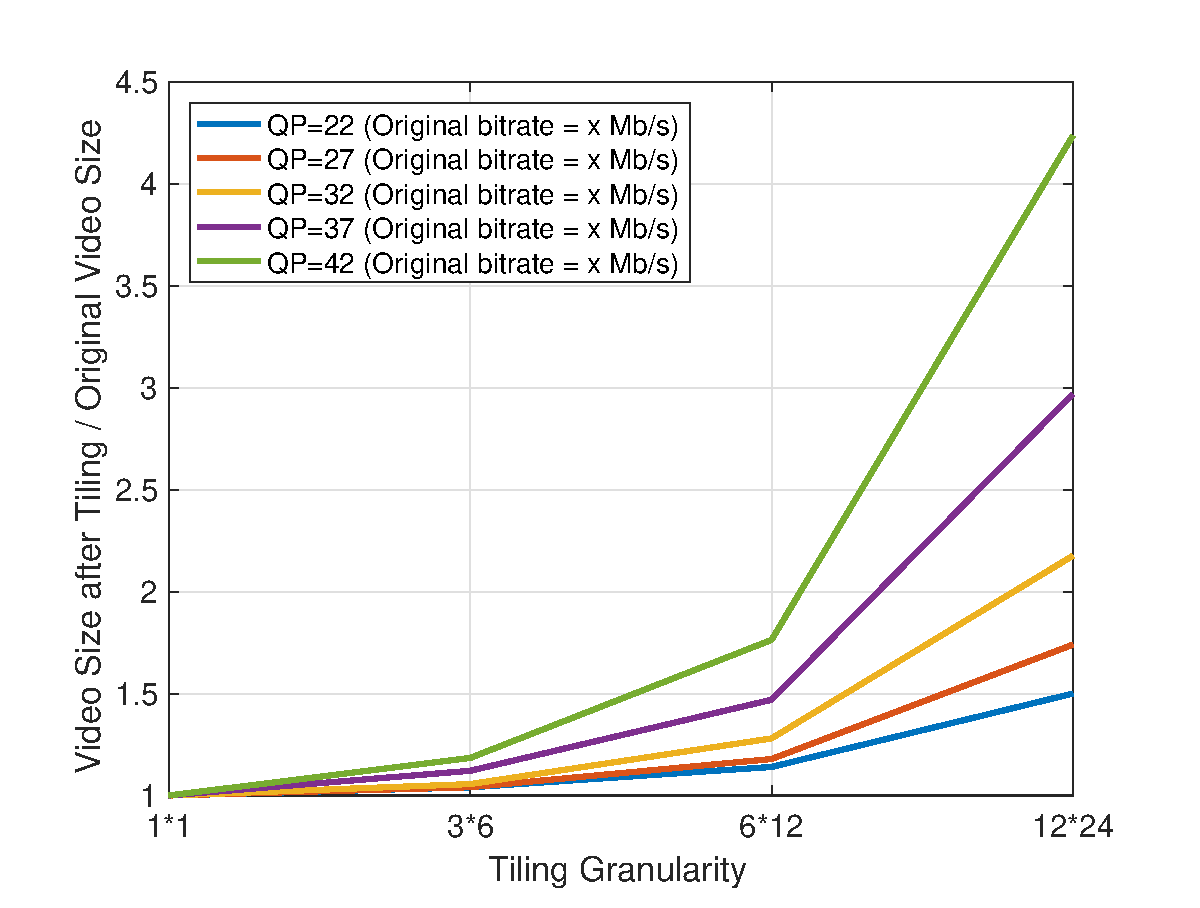
\includegraphics[width=2.5in]{images/bitrateefficiency.eps}
  \caption{The ratio of video size after tiling and original video size in each tiling granularity and each bitrate level. We notice that fine-grained tiling introduces serious bitrate efficiency problem, especially in low bandwidth situations in which the overall bitrate of each tile is low.}
  \label{bitrateefficiency}
  \end{figure}

\textbf{Challenge 3: Information needed for perceived quality computation is disparted on server-side and client-side.} 

To optimize perceived quality, client needs to compute the perceived quality of each bitrate allocation and then make decision. However, different from video quality which only related to video content itself, perceived quality depends on both video content and user behavior. Information of video content is located on server-side while information of user behavior is located on client-side. To get information of video content with current DASH, client has to pre-request in information of each pixel from server. This communication overload even exceed the overload of actual video streaming.

\subsection{Potential improvement}

As we have stated that perceived quality is not only related to object-viewpoint distance, it is also related to many factors, we need to clarify how much potential improvement can we get by taking above insights.

We set up a trace-driven experiment to evaluate this potential improvement. PSPNR[] is applied as a metric to measure perceived quality. Real traces are collected from over 800 VR displays of 48 users. In our experiment, each video has 5 different bitrate level. We compare the performance of 3 methods:

\begin{itemize}

\item \emph{Viewpoint-driven VR streaming.} Video is cut into 6*12 spatial rectangular tiles. Tiles on user's viewpoint is allocated the high bitrate. For other tiles, bitrate is allocated linearly decreasing with its distance to user's viewpoint.

\item \emph{Perceived quality driven VR streaming.} Suppose we can freely allocate bitrate to each spatial part of video without video tiling. With consideration of user viewpoint, content luminance and texture complexity, we do adaptive streaming to maximize user-perceived quality.

\item \emph{Perceived quality driven VR streaming. (with 3 VR factors)} Suppose we can freely allocate bitrate to each spatial part of video without video tiling. Besides user viewpoint, content luminance and texture complexity, we also take consideration of viewpoint moving speed, content Depth-of-Field and light / dark adaptation, we do adaptive streaming to maximize user-perceived quality.

\end{itemize}

\begin{figure}
  \centering
  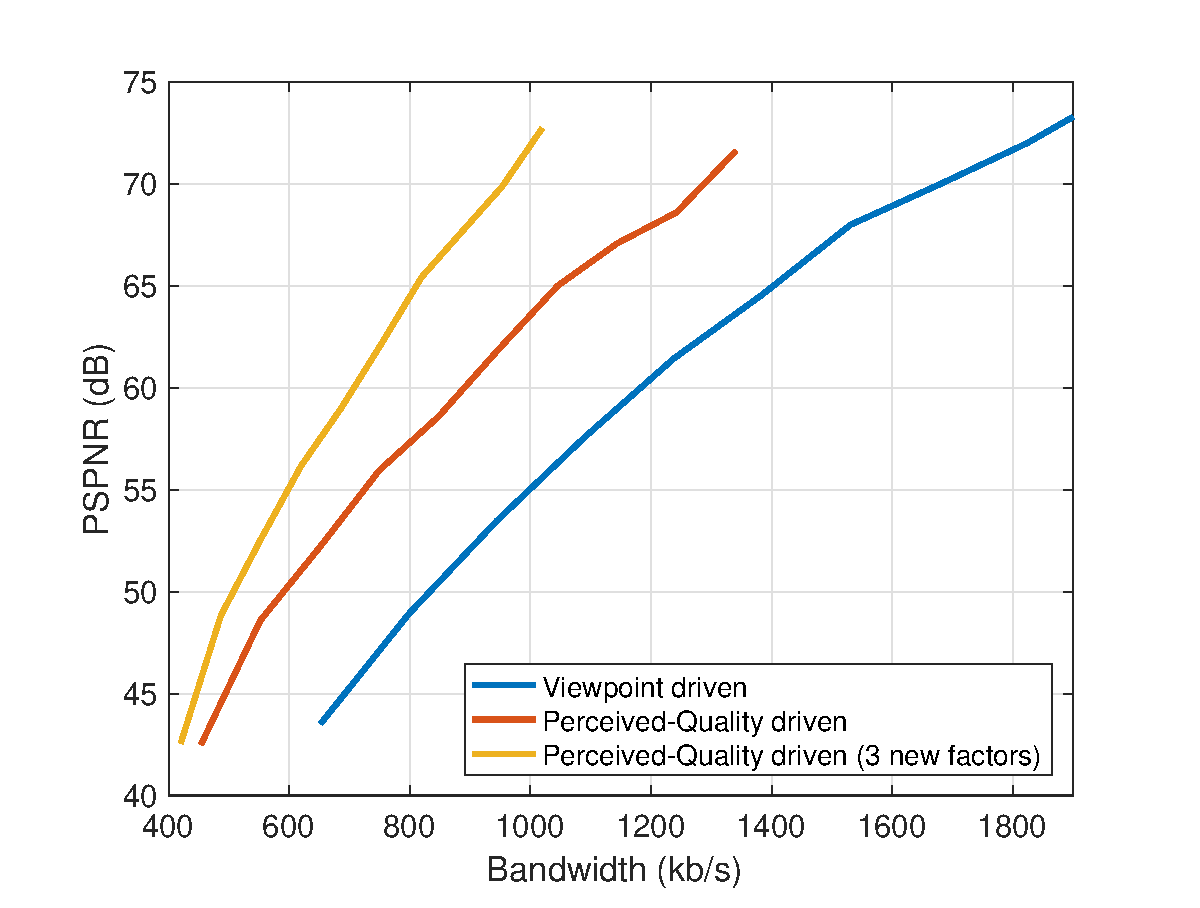
\includegraphics[width=2.5in]{images/improvement.eps}
  \caption{PSPNR-bandwidth tradeoff of (1) Viewpoint-driven VR streaming. (2) Perceived quality driven VR streaming. (3) Perceived quality driven VR streaming. (with 3 VR factors)}
  \label{potential1}
  \end{figure}

Fig. \ref{potential1} shows the PSPNR-bandwidth tradeoff of 3 strategies.

\textbf{Key observations:} 
\begin{itemize}
\item With consideration of content luminance and texture complexity, perceived-quality-driven VR streaming can save 30\% bandwidth compared with viewpoint-driven VR streaming providing the same PSPNR. Moreover, when we take consideration of viewpoint moving speed, object Depth-of-Field and light / dark adaptation, we can further save 20\% bandwidth.
\end{itemize}